% shall we have a discussion section after methods and results?
% Discussion
% 	- possibility of using the "domination graph" as data,
% 	where decks are nodes and win rates are the directed
% 	edges
% 	- there is some correlation in the win rate dictionary
% 	distribution, as cards appear alongside other cards
% 	- we don't use a Hessian or Jacobian based opt method,
% 	which would have been useful to understand sensitivity

To achieve the goals outlined in the introduction, {\sc Ludus} contains an auto battler game with a number of special cards with extra mechanics and a basic `vanilla' card that only engages in standard combat without extra mechanics. The details of these cards and their mechanics are explained below in Section~\ref{sec:ab-game-def}. The health and attack values of all cards can be adjusted as well as some values pertaining to the extra mechanics (such as how much damage to deal to an opponent's card when a card dies). Multiple cards of the same type that have different attack, health, or other values can be considered in the same game. 

Beyond the auto battler itself, {\sc Ludus} also contains an optimization framework to find configurations of available cards that are balanced, fair, and fun. These criteria are obviously quite subjective; so game designers can easily plug new metrics into the existing framework as they develop new ways of capturing their goals and preferences describing the metagame. This paper explores a few options as well.

\subsection{Playtesting Simulator} \label{sec:sim}

To serve as a data source for quantitative analysis, we create
a playtesting simulator for an original auto battler game we designed. 
This simulator is designed for research purposes, allowing the user to 
create cards with new mechanics and run tournaments between
arbitrary decks. 

All cards are equally available to all players, and there are no restrictions on the number of copies of a card allowed in players' decks or in the entire game. Some auto battlers have a drafting process in which cards are selected or purchased from a pool, but drafting and/or deck-building take different forms across different games \cite{hearthstone-battlegrounds,storybook-brawl,feh-pawnsOfLoki-video}. We do not explore variants of these processes in this paper, but we will consider them in future work.

\subsubsection{Card Definition} \label{sec:ab-game-def}

Cards have positive integer statistics including health points, 
attack, and parameters pertaining to a special mechanic. In our game, such special parameters
include the following:

% consider table instead of bullets for space
\begin{description}
	\item[Explosion Damage] When the card dies, it damages
	each of the opponent's cards by this many health points.
	\item[Heal Amount] Prior to entering combat, the card 
	restores this many health points to its player's rightmost
	card
	\item[Attack Growth Per Hit] When the card takes damage, its
	attack increases by this many points.
	\item[Explosion Heal] When the card dies, it heals
	each of its player's other cards by this many health points.
	\item[Heal Donation Percent] When the card would be healed,
	it instead restores this many percent of the health points
	to itself and donates the remaining health points to its
	player's other cards evenly.
	\item[Armor Points] The card starts with this many armor points.
	When the card would be damaged, it instead loses an armor point.
	When the card has zero armor points, it is damaged normally.
	\item[Damage Split Percent] When the card would be damaged,
	it instead receives this many percent of the damage to itself
	and splits the remaining damage evenly to its player's other cards.
	\item[Middle Age] Prior to entering combat, the card increases its
	attack by 1 if it has not participated in this many combat phases.
	After this many combat phases, the card decreases its attack by 1
	before entering combat.
	\item[Target Age] When the card dies, if it participated in this many
	combat phases, it deals this many damage points to each of the opponent's
	cards. If the card participated in fewer than this many combat phases, 
	it heals each of its player's other cards by health points equal to the
	number of combat phases in which the card participated.
	\item[Detonation Time] When the card has been healed or damaged this
	many times, the card and its opponent's card both die.
\end{description}

Other card mechanics without parameters include the copying the 
attack of the opponent's cards (morphing enemies) and swapping 
its health points and attack whenever its attack is greater than its health 
points (survivalist).

\subsubsection{Match Procedure} \label{sec:game}

Gameplay proceeds as follows in the simulator:

\begin{enumerate}
	\item Each player in a tournament selects an ordered list
	of cards to be their deck.
	\item Prior to combat, arrange the deck's cards left-to-right.
	\item Each combat phase pits the leftmost surviving card
	of each player against each other. The cards take damage equal to %by 
	%reducing their health points by
        their opponent card's attack.
	Cards with zero or fewer health points die, and surviving cards
	are rearranged to be the rightmost card of their respective decks.
	\item Repeat the combat phase until one or fewer players has a surviving card
	or the maximum number of combat phases has been reached.
	If both or neither players have at least one surviving card, the game is a draw.
	Otherwise, the player with a surviving card wins.
\end{enumerate}

\subsubsection{Win Rate Approximation} \label{sec:tourney}

We run a round-robin tournament where each deck plays one match against every other deck.
Unfortunately, for $n$ decks, this results in $n(n-1)/2 = n^2/2 - n/2$ matches. This quickly becomes prohibitively large to simulate. We developed an approximation algorithm that runs a subset of the games in order to estimate the win rates of cards and decks. It
randomly partitions the decks into groups of uniform size and runs round-robin tournaments within these groups.
For a group tournament with $k$ groups and $n$ total decks, this results in an upper bound of $k \cdot (n/k)(n/k - 1)/2 = n^2/(2k) - n/2$ matches in the case where 
$n$ is divisible by $k$.

\subsection{Metrics} \label{sec:metrics}

Quantitative measures of metagame health are needed to guide 
card statistic optimization. We present metrics built upon the
output data of the playtesting simulator.

The playtesting simulation outputs a data vector $v$.
Each entry $v_i \in [-1, 1]$ represents the average payoff of
the deck at index $i$ during the last round of playtesting in
the optimization process. A payoff of 1 indicates a win. A
payoff of 0 means a tie, and a loss results in a payoff of -1.
The average of these payoffs over the course of the simulated
tournament for a deck make up the entries of $v$.

We then transform $v$ into another vector of length $n$ that maps a card to the
average win rate of the decks in which the card appears. This
vector $w$ has entries
$w_j \in [0, 1]$, the average win rate of the decks in which
the card at index $j$ appears. We present three metrics that 
evaluate the uniformity of %use
this distribution of win rates among the cards.

\subsubsection{Per-card Payoff}

\begin{equation}
	\mathrm{PCP} = \frac{1}{n} \sum_j \left|\mathrm{payoff}(w_j)\right|^2
\end{equation}

Since average payoffs are equal to 0 when a deck wins as many matches as it loses, this is a metric to 
minimize if we want to punish overly competitive or terrible decks.

\subsubsection{Standard Deviation Metric}

\begin{equation}
	\mathrm{SDM} = \sqrt{\frac{1}{n} \sum_j \left|w_j - \left(\frac{1}{n}\sum_j w_j\right)\right|^2}
\end{equation}

Minimizing standard deviation of the win rates may avoid cards with
drastically higher or lower win rates compared to other cards.

\subsubsection{Entropy Metric}

\begin{equation}
	\mathrm{EM} = -\sum_j \frac{w_j}{\sum_j w_j} \log\left(\frac{w_j}{\sum_j w_j}\right)
\end{equation}

%Entropy of the win rates is a metric we may seek to maximize.
When the entropy of the win rates is maximized, we approach a uniform
distribution of win rates over the cards.

\subsubsection{Other Metrics} \label{sec:othermetrics}

The {\sc Ludus} framework is flexible; researchers and designers alike may develop their own metrics corresponding to their
own ideas of what constitutes a healthy metagame. For example, a game designer may know from historical data that
a certain distribution of win rates over cards or decks correspond to a period of celebrated parity in the metagame. 
The designer could conceivably use the Wasserstein distance or Kullback-Leibler 
divergence between this historical distribution and another distribution as a metric. Minimizing this metric 
might maintain similar levels of parity through future iterations of card releases.
Metrics could also evaluate other measurable elements like average turns per match.

\subsection{Optimization} \label{sec:optimization}

We use the PyGAD python library \cite{gad2021pygad} for genetic %optimization
algorithms. This searches for the optimal values of
specified parameters, which may include health points, attack, and special parameters, with respect to %that optimizes
the chosen metric.

We constrain the genetic algorithm to consider integer values between 1 and 10, inclusive. While hyperparameter tuning may have yielded better results,
we chose to run the genetic algorithm with 8 solutions and 4 parents mating per population for 32 generations in each experiment.

\subsection{Qualitative Analysis} \label{sec:qualitative-analysis}

Another way to understand the landscape of the metagame is through more qualitative methods. We look at two different ways of plotting data about the game results that give insights into the health and stability of the metagame. 

The first plot sweeps over two variables, typically of the same card, although not necessarily. This gives a visual representation of the metagame sensitivity under variations of a configuration, which can lead to some interesting insights about the relationships between cards.

\begin{figure}[t]
	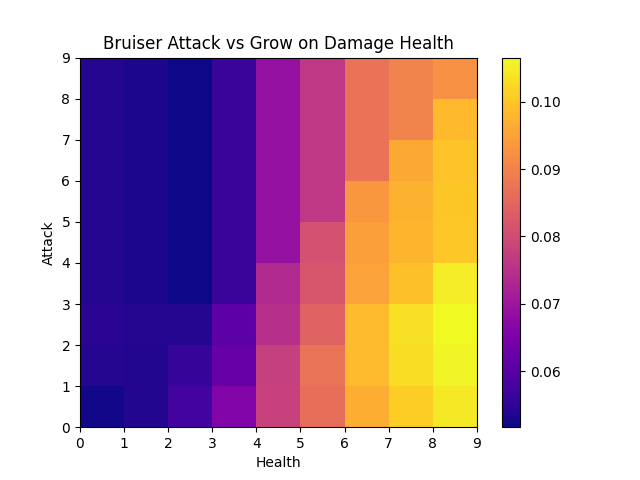
\includegraphics[width=10cm, height=8cm]{bruiser_vs_grow} 
	\caption{Plot showing how changes in the attack of the bruiser card and the health of the grow-on-damage card affect the metric value.}
	\label{fig:bruiser_vs_grow}
\end{figure}

Take, for example, the plot in Figure~\ref{fig:bruiser_vs_grow} of the value of the standard deviation metric given various values for the attack of the bruiser card and the health of the grow on damage card. The bruiser card is a vanilla card with a high attack (although variable in this situation) and one health point. The grow on damage card has a mechanic where each time it takes damage it gains one attack. Initially this card has one attack, and in this situation has a variable amount of health. If the grow on damage card is able to consistently become a powerful threat, it can become too strong and a necessity for high-level play, leading to an unbalanced metagame.

In the figure, we can see that configurations in the upper left corner, where the attack of the bruiser is greater than the health of the grow on damage card, tend to be much more favorable than the configurations in the lower right corner, where the opposite is true. This evidence supports the intuitive idea that the bruiser's high attack is a good counter to the grow on damage card because the bruiser card can quickly remove the grow on damage card before it has had enough interactions to grow its damage to a large number. This kind of information can be quite useful to a game designer, who can see very clearly that the inclusion of a high-damage card can improve the metagame dramatically if the grow on damage card is found to be too powerful.

The second plot is a histogram of the deck win rates after running a tournament amongst all possible decks. %, the win rates of each deck are plotted in a histogram.
The resulting distribution can have features that may be informative to human game designers. For example, examine the difference between the distributions %shown
in Figure~\ref{fig:special_only_dist_before} and Figure~\ref{fig:special_only_dist_after} from tournaments using two configurations of the same card parameters. 

% TODO: Continue generating more distribution plots, and with other metrics perhaps. And metric discrepancy between logs and pickle file. Investigate length of games.
\begin{figure}[t]
	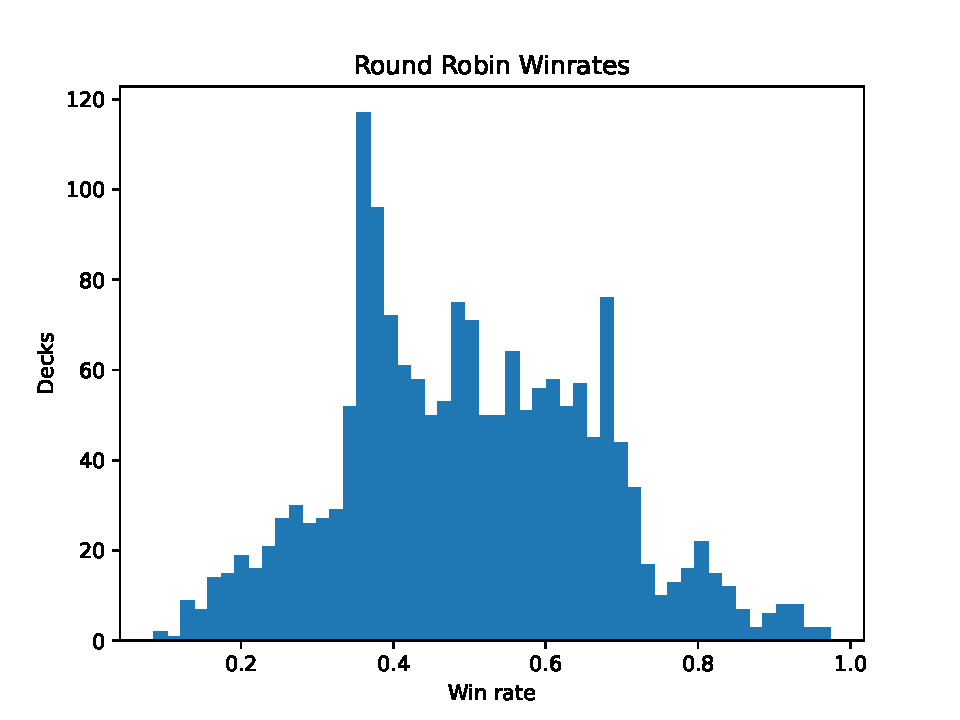
\includegraphics[scale=0.5]{special_only_4_5_8_8_4_8_3_3_3_5}
	\caption{Distribution of deck winrates before optimization. }
	\label{fig:special_only_dist_before}

	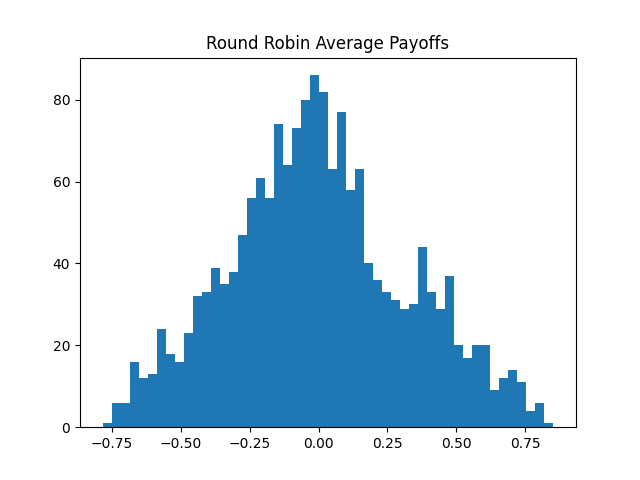
\includegraphics[scale=0.5]{special_only_1_3_4_3_3_1_7_8_5_7}
	\caption{Distribution of deck winrates after optimization. }
	\label{fig:special_only_dist_after}
\end{figure}

Given playtesting input from actual players and historical data from other successful metagames, game designers can interpret the %understand the what
changes new cards have brought and implement changes to the game or metrics for optimization that will improve the experience of human players.

\subsection{Experiment Design}

% in methods: only describe the phases of experiments in a high level -- 1. build decks 2. tournaments 3. ... their common pattern
% describe set up, techniques; write about analysis and numbers in results

Our experiments share common phases.

\begin{enumerate}
	\item Build decks. We generate a set of cards and their associated attack, health points, and special parameters.
	Depending on the experiment, a subset of these parameters may vary between simulations during the optimization process.
	From this set of cards, the decks are permutations of 3 cards from the set, allowing for duplicates.
	\item Run tournaments. This will be either be a group or a round-robin tournament as described in Section~\ref{sec:tourney}.
	\item Optimize. These tournaments are run within each iteration of our genetic algorithm to produce a metric estimating the best
	possible health of the metagame with respect to configurations of the card parameters. %of the built decks.
\end{enumerate}
